\documentclass[12pt,a4paper]{article}

\usepackage[english]{babel} 			%% englische Sprache

\usepackage[latin1,applemac]{inputenc}	%% deutsche Umlaute wie normale
 								%% Buchstaben verwenden
 								%% (ansonsten muesste � durch a getippt werden)
\usepackage{a4wide} 				%% kleinere Seitenr�nder

\usepackage{amssymb,amsthm,amsfonts, amsmath}
								%% diverse Matheerweiterungen, z.B. \implies
 								%% diverse Matheerweiterungen, z.B. \mathbb{R}
%\usepackage{stmaryrd} 				%% weitere Symbole
\usepackage{epsfig} 					%% um eps-Dateien einzubinden (\epsfig{file=...})
\usepackage{longtable} 				%% fuer Tabellen ueber mehrere Seiten
\usepackage{color}
\usepackage{hyperref}
\usepackage{dsfont}
\usepackage{caption}
\usepackage{multirow}
\usepackage{float}

\hypersetup{						%get rid of red box around hyperlink
pdfborder = {0 0 0}
}

\usepackage{listings} 				% noice code inclusion
\usepackage{color}
\usepackage{enumerate}


\definecolor{deepblue}{rgb}{0,0,0.5}
\definecolor{deepred}{rgb}{0.6,0,0}
\definecolor{deepgreen}{rgb}{0,0.5,0}
\lstset{
	frame=single,
	language=Python,
	belowcaptionskip=1\baselineskip,
	breaklines=true,
	frame=tb,
	showstringspaces=false,
	basicstyle=\footnotesize\ttfamily,
	keywordstyle=\color{deepblue},
	emphstyle=\color{deepred},    		% Custom highlighting style
	stringstyle=\color{deepgreen},
	commentstyle=\itshape\color{deepgreen}
}


\title{\textbf{ Programming project} \\ \textit{CS-E4600 - Algorithmic Methods of Data Mining}}
\author{H�ctor Laria Mantec�n and Maximilian Proll}
\date{\today}

\begin{document}

\maketitle

%\begin{abstract}
%
%\end{abstract}

\section{Exact computation}


\begin{table}[h!]
\centering
\caption{\textbf{Exact statistics} for both directed and undirected version of the networks as well as running time}
\begin{tabular}{c|c|c|c|c}
	& \textbf{wiki-Vote}	& \textbf{soc-Epinions1}	& \textbf{ego-Gplus}	&	\textbf{soc-Pokec}\\ \hline
directed \textbf{LSCC}	& 	& 	& 	&	\\ \hline
\textbf{\# of nodes} 		&1.300 			&32.223				&N/A				&N/A	\\
\textbf{\# of edges} 		&39.456 			&443.506				&N/A				&N/A	\\
\textbf{median} 			&3	 			&4					&N/A				&N/A	\\
\textbf{mean} 			&2,877 			&4,405				&N/A				&N/A	\\
\textbf{diameter} 		&9	 			&16					&N/A				&N/A	\\
\textbf{effective diameter} 	&4	 			&6					&N/A				&N/A	\\
\textbf{running time nX}	&28s				&					&N/A				&N/A	\\
\textbf{running time gt}	&8s				&3h 49min 14s			&N/A				&N/A	\\ \hline
undirected \textbf{LWCC}	& 	& 	& 	&	\\ \hline
\textbf{\# of nodes} 		&7.066 			&75877				&N/A				&N/A	\\
\textbf{\# of edges} 		&103.663			&508836				&N/A				&N/A	\\
\textbf{median} 			&3	 			&4					&N/A				&N/A	\\
\textbf{mean} 			&3,247 			&4,308				&N/A				&N/A	\\
\textbf{diameter} 		&7	 			&15					&N/A				&N/A	\\
\textbf{effective diameter} 	&4	 			&5					&N/A				&N/A	\\
\textbf{running time nX} 	&9min 25s		&					&N/A				&N/A	\\
\textbf{running time gt} 	&1min 50s		&8h 52min 49s			&N/A				&N/A
\end{tabular}
\label{tab:exactstatistics}
\end{table}



\section{Approximate Computation}

\subsection{Computation of approximations for a fixed accuracy parameter for all three approximation techniques}

\begin{table}[h!]
\centering
\caption{Approximate statistics for \textbf{random sampling pairs of vertices} for both directed and undirected version of the networks as well as running time}
\begin{tabular}{c|c|c|c|c}
	& \textbf{wiki-Vote}	& \textbf{soc-Epinions1}	& \textbf{ego-Gplus}	&	\textbf{soc-Pokec}\\ \hline
accuracy	& 10\% 	&5\% 	& 	&	\\ \hline
directed \textbf{LSCC}	& 	& 	& 	&	\\ \hline
%\textbf{\# of nodes} 		&1.300 			&32.223				&N/A				&N/A	\\
%\textbf{\# of edges} 		&39.456 			&443.506				&N/A				&N/A	\\
\textbf{median} 			&3	 			&4					&N/A				&N/A	\\
\textbf{mean} 			&2,869 			&4,387				&N/A				&N/A	\\
\textbf{diameter} 		&6	 			&9					&N/A				&N/A	\\
\textbf{effective diameter} 	&4	 			&6					&N/A				&N/A	\\
%\textbf{running time nX}	&				&					&N/A				&N/A	\\
\textbf{running time gt}	&1s				&1min 20s			&N/A				&N/A	\\ \hline
undirected \textbf{LWCC}	& 	& 	& 	&	\\ \hline
%\textbf{\# of nodes} 		&7.066 			&75877				&N/A				&N/A	\\
%\textbf{\# of edges} 		&103.663			&508836				&N/A				&N/A	\\
\textbf{median} 			&3	 			&4					&N/A				&N/A	\\
\textbf{mean} 			&3,283 			&4,328				&N/A				&N/A	\\
\textbf{diameter} 		&6	 			&9					&N/A				&N/A	\\
\textbf{effective diameter} 	&4	 			&5					&N/A				&N/A	\\
%\textbf{running time nX} 	&				&					&N/A				&N/A	\\
\textbf{running time gt} 	&5s				&7min 54s			&N/A				&N/A
\end{tabular}
\label{tab:approximatestatistics_randomsample}
\end{table}

\begin{table}[h!]
\centering
\caption{Approximate statistics for \textbf{breadth-first search on random sources} for both directed and undirected version of the networks as well as running time}
\begin{tabular}{c|c|c|c|c}
	& \textbf{wiki-Vote}	& \textbf{soc-Epinions1}	& \textbf{ego-Gplus}	&	\textbf{soc-Pokec}\\ \hline
accuracy	&  	& 	& 	&	\\ \hline
directed \textbf{LSCC}	& 	& 	& 	&	\\ \hline
%\textbf{\# of nodes} 		&1.300 			&32.223				&N/A				&N/A	\\
%\textbf{\# of edges} 		&39.456 			&443.506				&N/A				&N/A	\\
\textbf{median} 			&	 			&					&N/A				&N/A	\\
\textbf{mean} 			&	 			&					&N/A				&N/A	\\
\textbf{diameter} 		&	 			&					&N/A				&N/A	\\
\textbf{effective diameter} 	&	 			&					&N/A				&N/A	\\
\textbf{running time nX}	&				&					&N/A				&N/A	\\
\textbf{running time gt}	&				&					&N/A				&N/A	\\ \hline
undirected \textbf{LWCC}	& 	& 	& 	&	\\ \hline
%\textbf{\# of nodes} 		&7.066 			&75.877				&N/A				&N/A	\\
%\textbf{\# of edges} 		&103.663			&508.836				&N/A				&N/A	\\
\textbf{median} 			&	 			&					&N/A				&N/A	\\
\textbf{mean} 			&	 			&					&N/A				&N/A	\\
\textbf{diameter} 		&	 			&					&N/A				&N/A	\\
\textbf{effective diameter} 	&	 			&					&N/A				&N/A	\\
\textbf{running time nX} 	&				&					&N/A				&N/A	\\
\textbf{running time gt} 	&				&					&N/A				&N/A
\end{tabular}
\label{tab:approximatestatistics_BFS}
\end{table}


\begin{table}[h!]
\centering
\caption{Approximate statistics for \textbf{the Flajolet-Martin algorithm} for both directed and undirected version of the networks as well as running time}
\begin{tabular}{c|c|c|c|c}
	& \textbf{wiki-Vote}	& \textbf{soc-Epinions1}	& \textbf{ego-Gplus}	&	\textbf{soc-Pokec}\\ \hline
accuracy	&  	& 	& 	&	\\ \hline
directed \textbf{LSCC}	& 	& 	& 	&	\\ \hline
%\textbf{\# of nodes} 		&1.300 			&32.223				&N/A				&N/A	\\
%\textbf{\# of edges} 		&39.456 			&443.506				&N/A				&N/A	\\
\textbf{median} 			&	 			&					&N/A				&N/A	\\
\textbf{mean} 			&	 			&					&N/A				&N/A	\\
\textbf{diameter} 		&	 			&					&N/A				&N/A	\\
\textbf{effective diameter} 	&	 			&					&N/A				&N/A	\\
\textbf{running time nX}	&				&					&N/A				&N/A	\\
\textbf{running time gt}	&				&					&N/A				&N/A	\\ \hline
undirected \textbf{LWCC}	& 	& 	& 	&	\\ \hline
%\textbf{\# of nodes} 		&7.066 			&75.877				&N/A				&N/A	\\
%\textbf{\# of edges} 		&103.663			&508.836				&N/A				&N/A	\\
\textbf{median} 			&	 			&					&N/A				&N/A	\\
\textbf{mean} 			&	 			&					&N/A				&N/A	\\
\textbf{diameter} 		&	 			&					&N/A				&N/A	\\
\textbf{effective diameter} 	&	 			&					&N/A				&N/A	\\
\textbf{running time nX} 	&				&					&N/A				&N/A	\\
\textbf{running time gt} 	&				&					&N/A				&N/A
\end{tabular}
\label{tab:approximatestatistics_Flajolet-Martin}
\end{table}

\newpage
asd

\newpage

\subsection{Approximation of the network statistics for different values of the accuracy parameter}

\begin{figure}[h!]
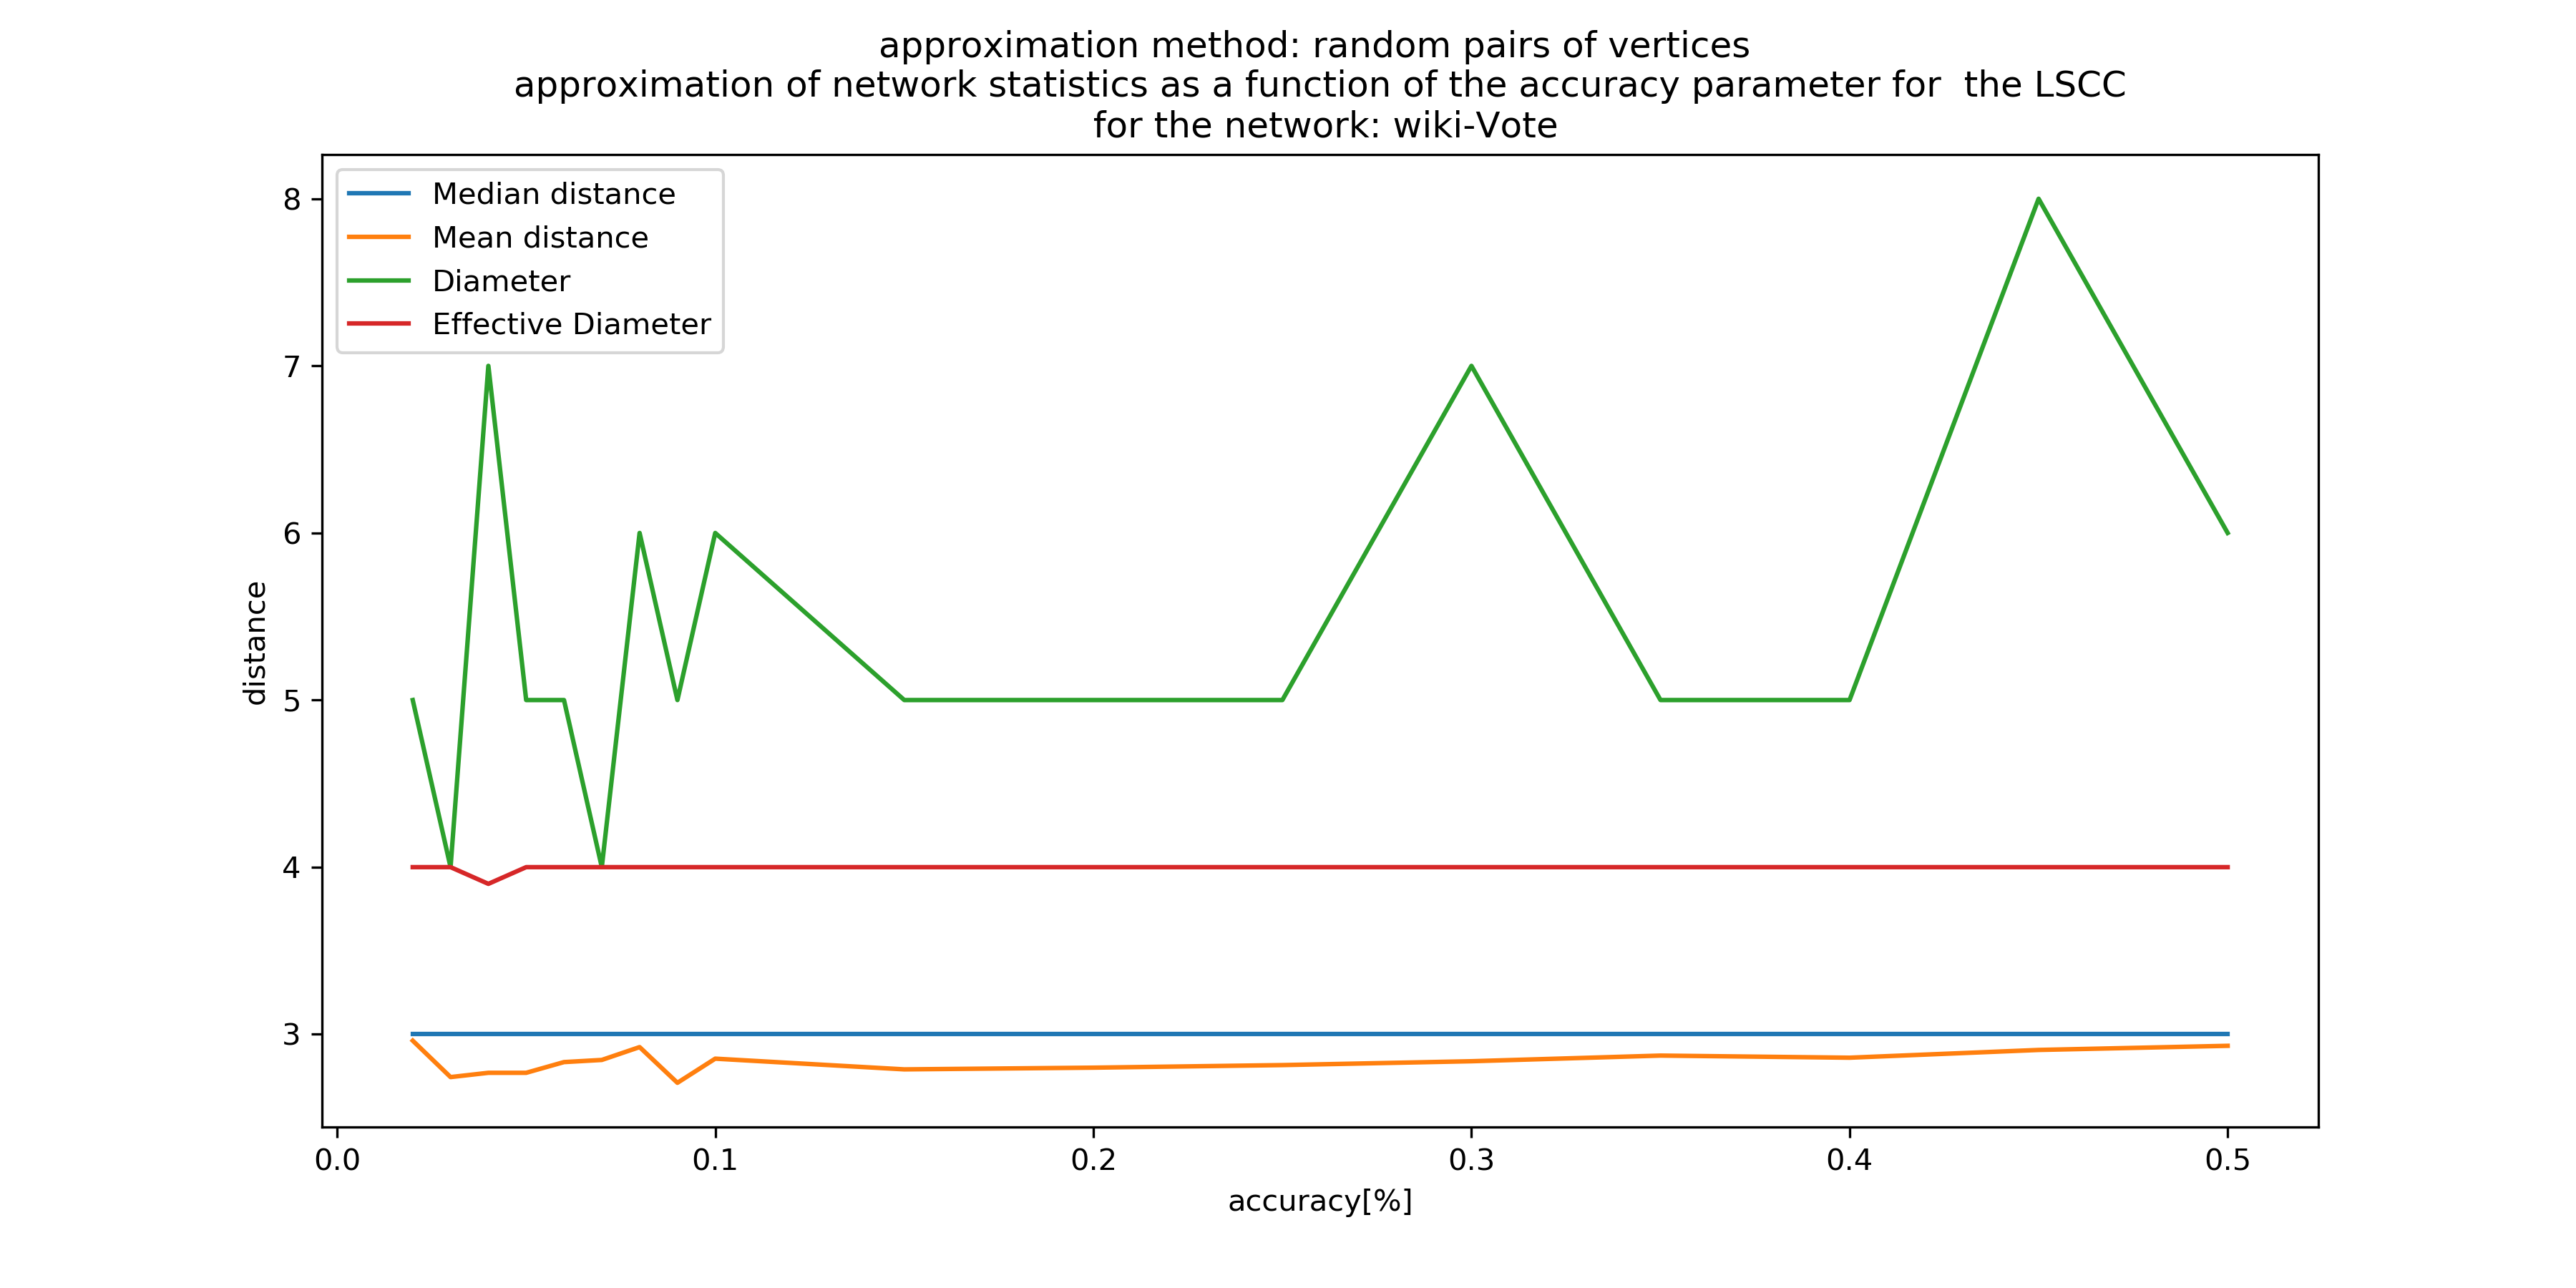
\includegraphics[width=0.9\linewidth]{figures/2_2_wiki-Vote_lscc.png}
\caption{First approximation of the network statistics by \textbf{sampling random pairs of vertices} to approximate network statistics as a function of the accuracy parameter for the \textbf{LSCC} for the network \textit{wiki-Vote}}
\label{pic:2_2_wiki-Vote_lscc}
\end{figure}

\begin{figure}[h!]
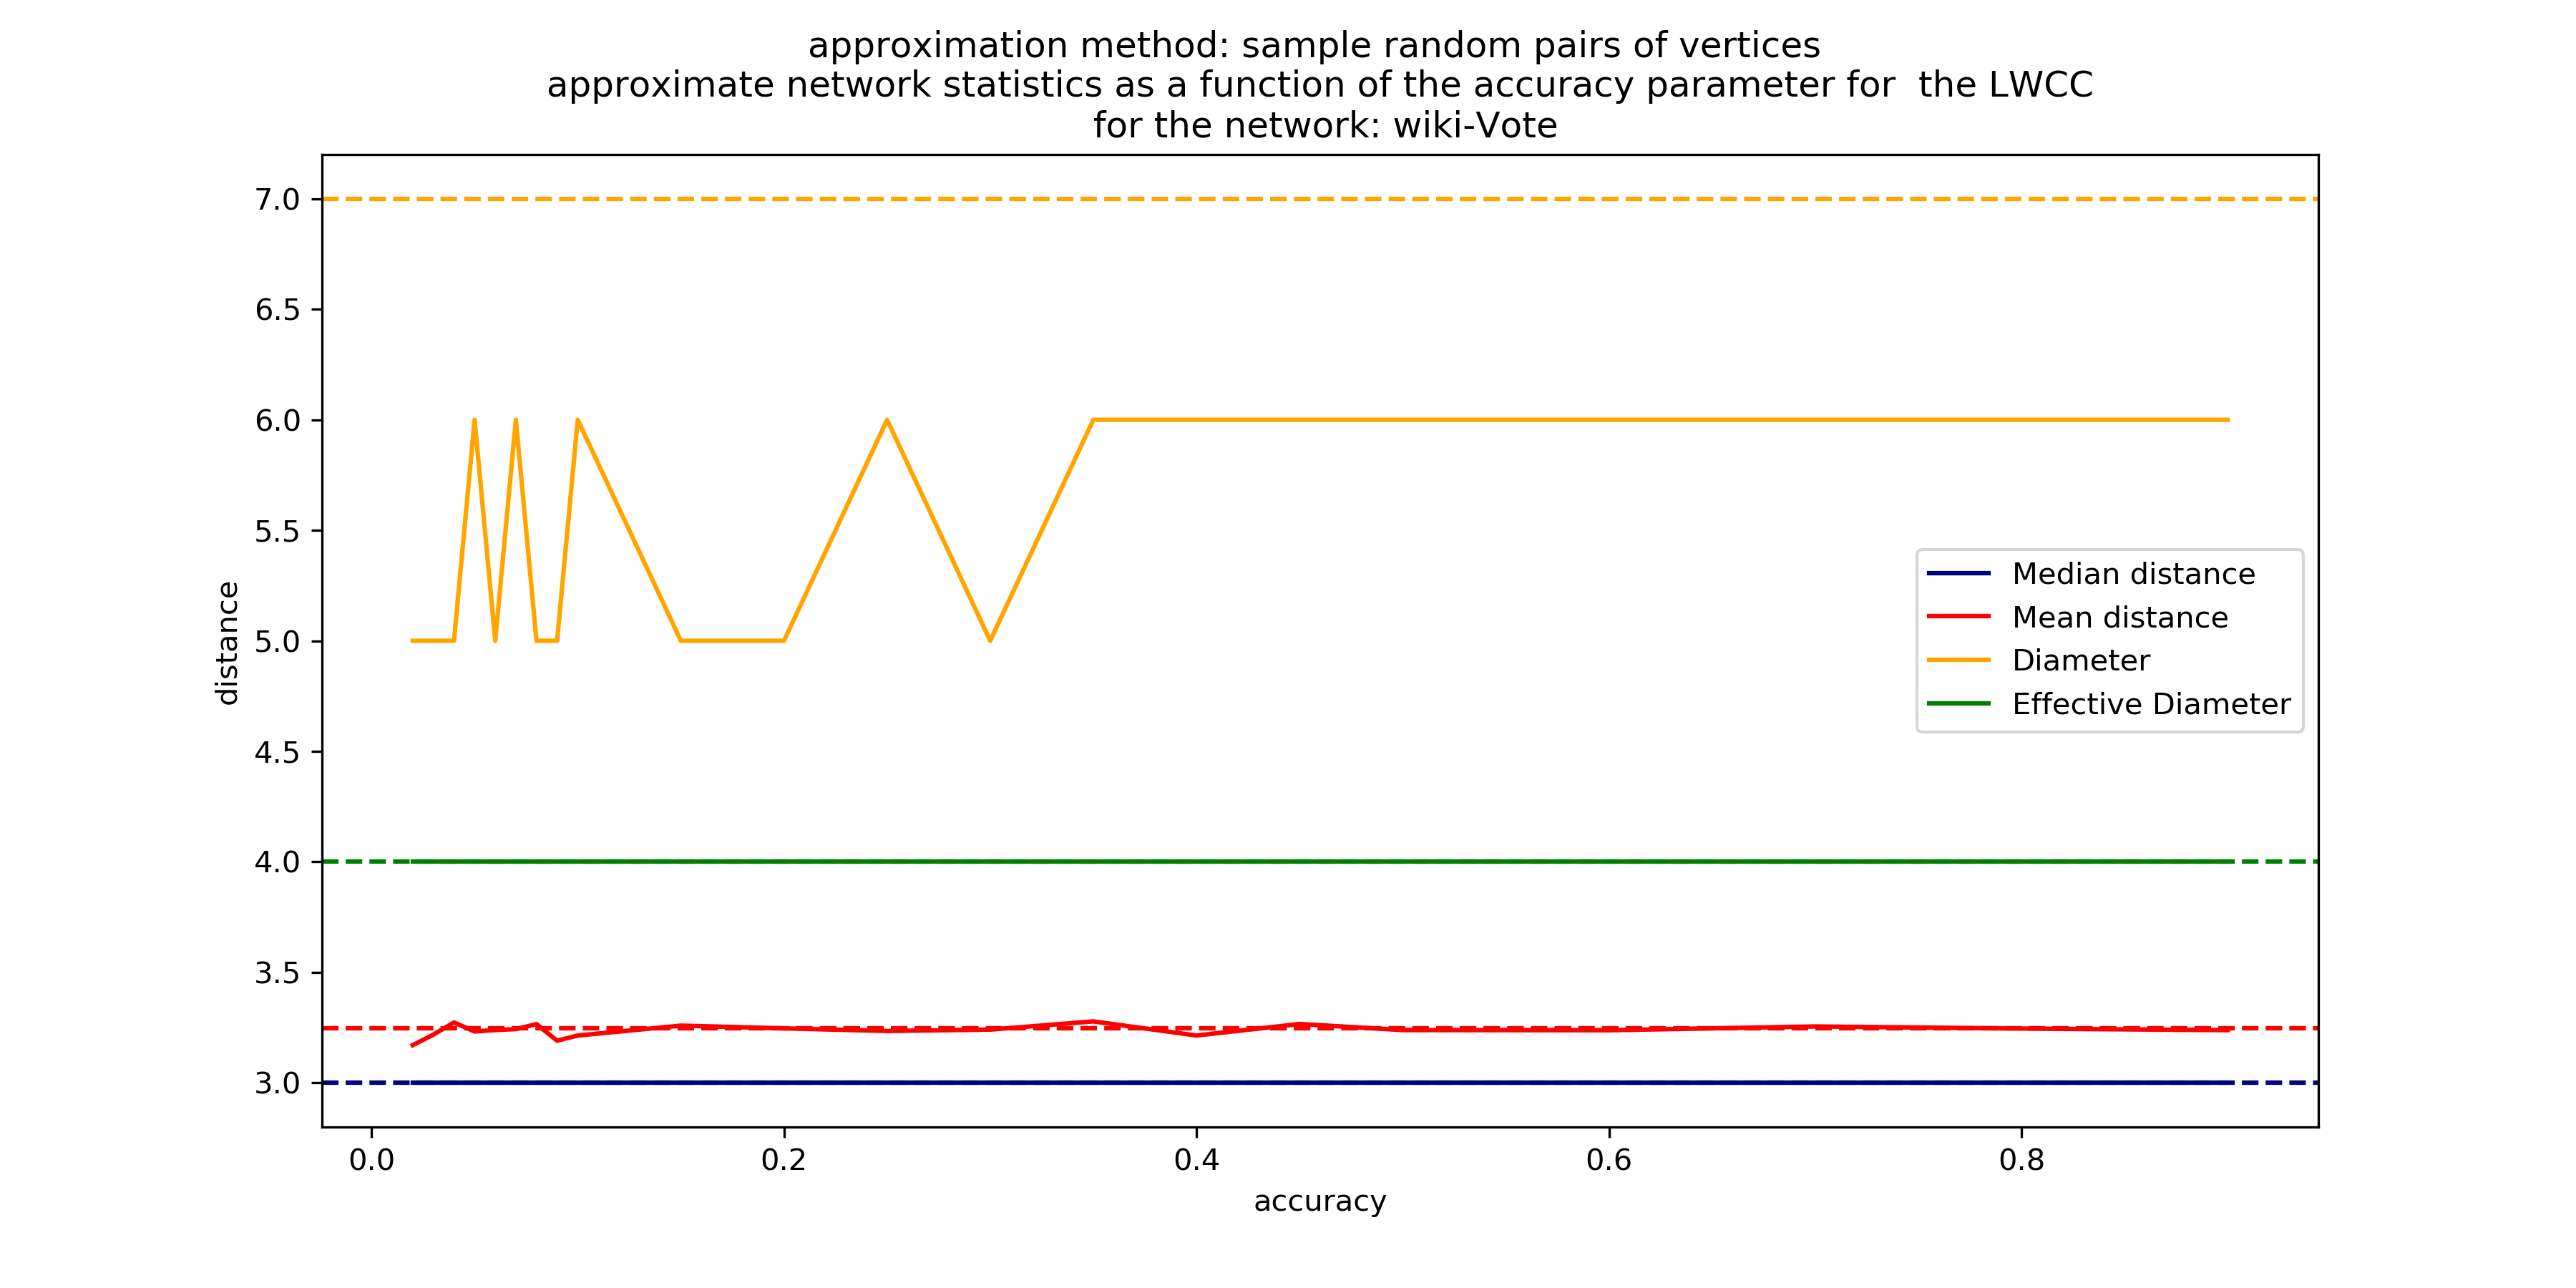
\includegraphics[width=0.9\linewidth]{figures/2_2_wiki-Vote_lwcc.png}
\caption{First approximation of the network statistics by \textbf{sampling random pairs of vertices} to approximate network statistics as a function of the accuracy parameter for the \textbf{LWCC} for the network \textit{wiki-Vote}}
\label{pic:2_2_wiki-Vote_lwcc}
\end{figure}


\subsection{Discussion}

\begin{enumerate}[(i)]
\item How good is the approximation?
\item Which of the three approximation methods is better and why?
\item What is the recommended value of the accuracy parameter, according to your experiments?
\end{enumerate}


\end{document}
